\chapter{Referencial Teórico}
\label{cap:referencial-reorico}

\section{O que é Machine Learning?}
\label{sec:oqueemachinelearning}

Não existe uma definição que seja aceita por todos, porem o principal objetivo de ML é identificar padrões e realizar ações, oque remete ao aprendizado,
que em sua base é identificar padrões e saber reconhece-los quando vê-los novamente. O processo básico de aprendizagem consiste em entrada de dados, abstração e generalização.
\begin{alineas}
	\item Entrada de dados: são fatos tirados da memoria ou da observação;
	\item Abstração: transformar estes dados em algo mais objetivo e que faça sentido;
	\item Generalização: utiliza os dados abstraídos e para  identificar padrões e assim classifica-los;			
\end{alineas}

\begin{figure}[h!]
	\centering
	\Caption{\label{fig:processo-aprendizagem} Fluxo do processo de aprendizagem.}	
	\UECEfig{}{
		\fbox{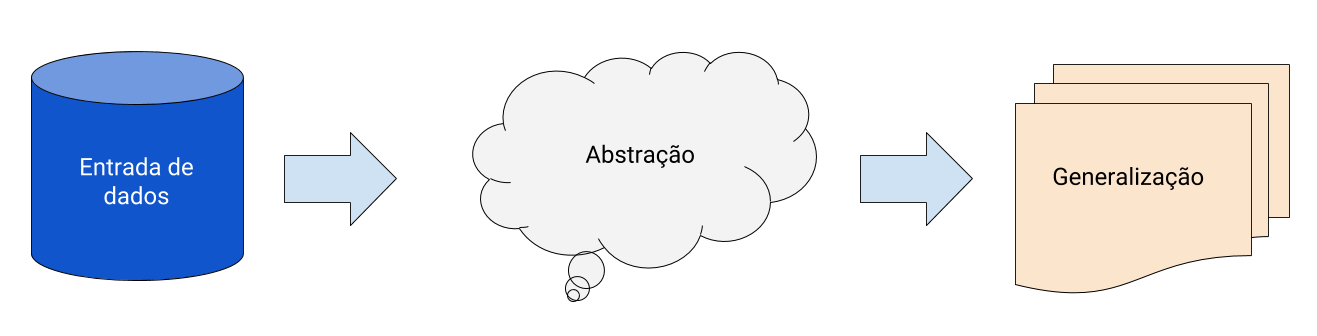
\includegraphics[width=15cm]{figuras/procc-learning}}
	}{
		\Fonte{Elaborado pelo autor}
	}	
\end{figure}

Todo este processo ocorre na ordem apresentada, pois o conceito de abstração e generalização estão muito próximos e tecnicamente um não faz sentido sem o outro. Os passos de abstração e generalização do processo de aprendizagem ocorrem subconscientemente em seres humanos, logo pode ser complexo representar este processo em linguagem computacional.


\subsection{Abstração e Representação de Dados}
\label{cap:abs-representacao-dados}

Durante a abstração os dados de entradas, são preparados para que possuam algum sentido em um contexto. Para ilustrar este processo, lembre de quando aprendeu a executar operações de soma e subtração, que sua professora apresentou o exemplo:
Uma maçã mais outra maçã é igual à duas maçãs, você deixou de lado todas as propriedades da maçã como ser uma fruta, ter a cor vermelha  ou possuir sementes, para um tipo de unidade , uma unidade de um tipo mais outra unidade do mesmo tipo é igual à duas unidades, ou seja para o contexto de soma não importa se é uma fruta ou a cor e sim a unidade.



%
%	\begin{figure}[h!]
%		\centering
%		\Caption{\label{fig:exemplo-1} Lorem ipsum dolor sit amet, consectetur adipiscing elit. Suspendisse commodo lectus et augue elementum varius.}	
%		\UECEfig{}{
%			\fbox{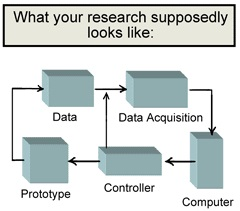
\includegraphics[width=8cm]{figuras/figura-1}}
%		}{
%			\Fonte{Elaborado pelo autor}
%		}	
%	\end{figure}
%	
%\lipsum[11]
%
%
%\section{Fundamentação Teórica B}
%\label{sec:fundamentacao-teorica-b}
%
%Integer non lacinia magna. Aenean tempor lorem tellus, non sodales nisl commodo ut. Proin mattis placerat risus sit amet laoreet. Praesent sapien arcu, maximus ac fringilla efficitur, vulputate faucibus sem. Donec aliquet velit eros, sit amet elementum dolor pharetra eget. Integer eget mattis %libero. Praesent ex velit, pulvinar at massa vel, fermentum dictum mauris. Ut feugiat accumsan augue, et ultrices ipsum euismod vitae
%
%	\begin{figure}[h!]
%		\centering
%		\Caption{\label{fig:exemplo-2} Maecenas luctus augue odio, sed tincidunt nunc posuere nec}	
%		\UECEfig{}{
%			\fbox{
\includegraphics[width=8cm]{figuras/figura-2}}
%		}{
%			\Fonte{Elaborado pelo autor}			
%		}	
%	\end{figure}
%
%Nunc ac pretium dui. Mauris aliquam dapibus nulla ac mattis. Aenean non tortor volutpat, varius lectus vitae, accumsan nibh. Cras pretium vestibulum enim, id ullamcorper tortor ultrices non. Integer sodales viverra faucibus. Curabitur at dui lacinia, rhoncus lacus at, blandit metus. Integer %scelerisque non enim quis ornare.
%
%\lipsum[13]

	\begin{table}[h!]	
		\centering
		\Caption{\label{tab:exemplo-1} Duis faucibus, enim quis tincidunt pellentesque, nisl leo varius nulla, vitae tempus dui mauris ac ante purus lorem}		
		\UECEtab{}{
			\begin{tabular}{cll}
				\toprule
				Ranking & Exon Coverage & Splice Site Support \\
				\midrule \midrule
				E1 & Complete coverage by a single transcript & Both splice sites\\
				E2 & Complete coverage by more than a single transcript & Both splice sites\\
				E3 & Partial coverage & Both splice sites\\
				E4 & Partial coverage & One splice site\\
				E5 & Complete or partial coverage & No splice sites\\
				E6 & No coverage & No splice sites\\
				\bottomrule
			\end{tabular}
		}{
		\Fonte{Elaborado pelo autor}
	}
	\end{table}

%Duis faucibus, enim quis tincidunt pellentesque, nisl leo varius nulla, vitae tempus dui mauris ac ante. Quisque purus lorem, pharetra sit amet lobortis eu, vehicula vitae purus. Ut varius, erat nec vehicula elementum, risus est tempus justo, nec vulputate augue leo egestas metus.
%
%	\begin{figure}[h!]
%		\centering
%		\Caption{\label{fig:exemplo-3} Ut posuere, ex quis sagittis auctor, magna massa euismod felis}	
%		\UECEfig{}{
%			\fbox{
\includegraphics[width=8cm]{figuras/figura-2}}
%		}{
%		\Fonte{Elaborado pelo autor}			
%	}	
%	\end{figure}
%
%\lipsum[14]
%
%	\begin{table}[h!]	
%		\centering
%		\Caption{\label{tab:exemplo-2} Etiam molestie, nulla a egestas aliquet, velit augue congue metus}		
%		\UECEtab{}{
%			\begin{tabular}{ccll}
%				\toprule
%				Quisque & pharetra & tempus & vulputate \\
%				\midrule \midrule
%				E1 & Complete coverage by a single transcript & Both splice sites\\
%				E2 & Complete coverage by more than a single transcript & Both splice sites\\
%				E3 & Partial coverage & Both splice sites & Both \\
%				E4 & Partial coverage & One splice site & Both \\
%				E5 & Complete or partial coverage & No splice sites & Both\\
%				E6 & No coverage & No splice sites\\
%				\bottomrule
%			\end{tabular}
%		}{
%		\Fonte{Elaborado pelo autor}
%	}
%	\end{table}
%	
%Duis faucibus, enim quis tincidunt pellentesque, nisl leo varius nulla, vitae tempus dui mauris ac ante. Quisque purus lorem, pharetra sit amet lobortis eu, vehicula vitae purus.
%\acrlong{DATASUS},\acrlong{DNV},\acrlong{DO},\acrlong{ESF},\acrlong{IBGE},\acrlong{MFC},\acrlong{MI},\acrlong{MS},\acrlong{NV},\acrlong{ODM},\acrlong{OI},\acrlong{OMS},\acrlong{ONU},\acrlong{PNI},\acrlong{PSF},\acrlong{RIPSA},\acrlong{RN},\acrlong{SIM},\acrlong{SINASC},\acrlong{SUS},\acrlong{TMI},%\acrlong{TMMFC}
%
%\begin{alineascomponto}
%	\item Integer non lacinia magna. Aenean tempor lorem tellus, non sodales nisl commodo ut
%	\item Proin mattis placerat risus sit amet laoreet. Praesent sapien arcu, maximus ac fringilla efficitur, vulputate faucibus sem. Donec aliquet velit eros, sit amet elementum dolor pharetra eget
%	\item Integer eget mattis libero. Praesent ex velit, pulvinar at massa vel, fermentum dictum mauris. Ut feugiat accumsan augue, et ultrices ipsum euismod vitae
%	\begin{subalineascomponto}
%		\item Integer non lacinia magna. Aenean tempor lorem tellus, non sodales nisl commodo ut
%		\item Proin mattis placerat risus sit amet laoreet.
%	\end{subalineascomponto}
%\end{alineascomponto}